% --- 1. PREAMBLE ---
\documentclass[11pt, a4paper]{article}

% --- Core Packages ---
\usepackage[a4paper, top=2.5cm, bottom=2.5cm, left=2cm, right=2cm]{geometry} % Page layout
\usepackage[T1]{fontenc} % Output font encoding
\usepackage{times}       % Use Times New Roman for text
\usepackage{mathptmx}  % Use Times-compatible fonts for math

% --- Additions for TikZ plots ---
\usepackage{pgfplots}
\pgfplotsset{compat=1.18}
\usepgfplotslibrary{fillbetween}

% --- Principle 3: Smart Package Loading ---
% We load only the packages necessary for the document's content.
\usepackage{amsmath}  % For math environments (equations, align, etc.)
\usepackage{booktabs} % For professional tables
\usepackage{listings} % For formatting code blocks
\usepackage{xcolor}   % For defining colors in listings
\usepackage{caption}  % For customizing captions
\usepackage[dvipsnames]{xcolor} % For more color names

% --- hyperref must be last (with few exceptions) ---
\usepackage{hyperref}

% --- 2. DOCUMENT CONFIGURATION ---

% Hyperlink setup
\hypersetup{
    colorlinks=true,
    linkcolor=blue,
    filecolor=magenta,      
    urlcolor=blue,
    citecolor=blue,
    pdftitle={A Primer on Wavelet Analysis},
    pdfauthor={A Guided Introduction},
}

% Code Listing setup (for Python)
\definecolor{codegreen}{rgb}{0,0.6,0}
\definecolor{codegray}{rgb}{0.5,0.5,0.5}
\definecolor{codeblue}{rgb}{0,0,0.8}
\definecolor{backcolour}{rgb}{0.95,0.95,0.95}

\lstdefinestyle{mystyle}{
    backgroundcolor=\color{backcolour},   
    commentstyle=\color{codegreen},
    keywordstyle=\color{magenta},
    numberstyle=\tiny\color{codegray},
    stringstyle=\color{codeblue},
    basicstyle=\ttfamily\footnotesize,
    breakatwhitespace=false,         
    breaklines=true,                 
    captionpos=b,                    
    keepspaces=true,                 
    numbers=left,                    
    numbersep=5pt,                  
    showspaces=false,                
    showstringspaces=false,
    showtabs=false,                  
    tabsize=2,
    language=Python
}
\lstset{style=mystyle}

% --- Title Information ---
\title{A Primer on Wavelet Analysis: \\ From Fourier's Limit to Practical Code}
\author{A Guided Introduction}
\date{\today}

% --- 3. DOCUMENT BODY ---
\begin{document}

\maketitle
\begin{abstract}
This document provides a comprehensive, yet accessible, introduction to the theory and application of Wavelet Analysis. We build intuition by starting with the limitations of the Fourier Transform, mathematically define the Continuous and Discrete Wavelet Transforms (CWT and DWT), and provide practical Python code examples for implementation.
\end{abstract}

\tableofcontents
\newpage

% --- NEW SECTION: INNER PRODUCT INTUITION ---
\section{Preamble: The Inner Product as a "Similarity" Engine}

Before we dive into \textit{why} we need wavelets, we must first understand the central mathematical tool that all ofthese transforms (including Fourier) are built on: the \textbf{inner product}.

Your intuition that the inner product measures "equi-directionality" is exactly correct. This idea can be extended from simple 2D vectors to infinitely-dimensional "vectors" we call functions.

\subsection{Intuition from Vectors}
In 2D, the inner product (or dot product) of $\vec{v}$ and $\vec{w}$ is:
$$ \vec{v} \cdot \vec{w} = |\vec{v}| |\vec{w}| \cos(\theta) $$
The key term is $\cos(\theta)$.
\begin{itemize}
    \item \textbf{High (Match):} If $\vec{v}$ and $\vec{w}$ point in the same direction, $\theta=0$ and $\cos(\theta)=1$. The inner product is at its positive maximum.
    \item \textbf{Zero (Unrelated):} If they are perpendicular (orthogonal), $\theta=90^\circ$ and $\cos(\theta)=0$. The inner product is zero.
    \item \textbf{Low (Unmatch):} If they point in opposite directions, $\theta=180^\circ$ and $\cos(\theta)=-1$. The inner product is at its negative maximum.
\end{itemize}

\subsection{Extending to Functions}
Now, imagine a function $f(t)$ is just a vector with an infinite number of "dimensions," where each point $t$ is a new dimension. How do we compute the inner product?

The dot product for discrete vectors is $\sum v_i w_i$. The continuous, infinite-dimensional equivalent of a sum ($\sum$) is an integral ($\int$).

Therefore, the inner product of two real functions $f(t)$ and $g(t)$ is:
$$ \langle f, g \rangle = \int_{-\infty}^{\infty} f(t) g(t) dt $$
This integral is just a single number. This number tells us \textit{exactly} the same thing as the vector dot product: how "similar" are the two functions?

\begin{itemize}
    \item \textbf{High (Match):} If $f(t)$ and $g(t)$ are "in sync" (where $f$ is positive, $g$ is positive; where $f$ is negative, $g$ is negative), their product $f(t)g(t)$ will be positive everywhere. The integral of all this positive area will be a \textbf{large positive number}.
    
    \item \textbf{Zero (Unrelated):} If $f(t)$ and $g(t)$ are "out of sync" (they are orthogonal), the product $f(t)g(t)$ will have exactly as much positive area as it has negative area. The integral of these cancelling areas will be \textbf{zero}.
    
    \item \textbf{Low (Unmatch):} If $f(t)$ and $g(t)$ are "perfectly opposite" (where $f$ is positive, $g$ is negative), their product $f(t)g(t)$ will be negative everywhere. The integral of all this negative area will be a \textbf{large negative number}.
\end{itemize}

\begin{figure}[htbp]
\centering
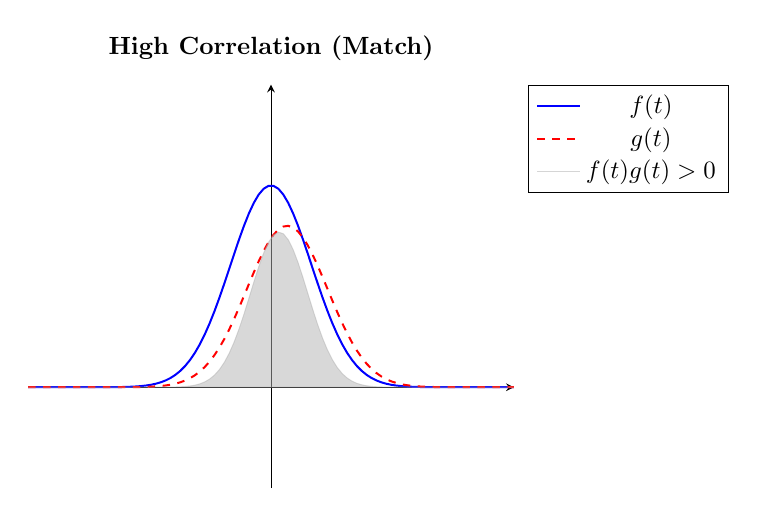
\begin{tikzpicture}[scale=0.9]
\begin{axis}[
    title={\textbf{High Correlation (Match)}},
    axis lines=middle, xtick=\empty, ytick=\empty,
    xmin=-3, xmax=3, ymin=-0.5, ymax=1.5,
    legend pos=outer north east]
    
    \addplot[blue, thick, domain=-3:3, samples=100] {exp(-2*x^2)}; \addlegendentry{$f(t)$};
    \addplot[red, dashed, thick, domain=-3:3, samples=100] {0.8*exp(-2*(x-0.2)^2)}; \addlegendentry{$g(t)$};
    
    % Plot the product f(t)g(t) and fill to axis
    \addplot[black!30, fill=black!30, opacity=0.5, domain=-3:3, samples=100] {exp(-2*x^2) * 0.8*exp(-2*(x-0.2)^2)} \closedcycle;
    \addlegendentry{$f(t)g(t) > 0$};
\end{axis}
\end{tikzpicture}
\caption{When $f(t)$ and $g(t)$ are "in sync," their product $f(t)g(t)$ is always positive, leading to a large positive integral.}
\end{figure}

\begin{figure}[htbp]
\centering
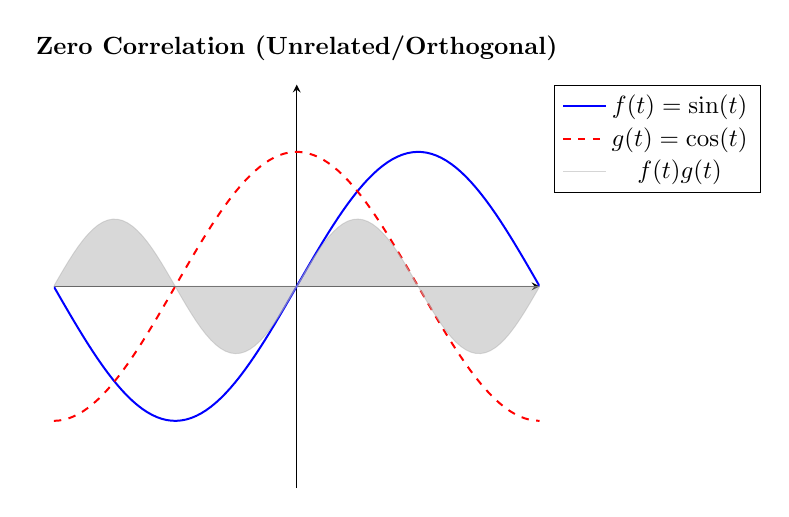
\begin{tikzpicture}[scale=0.9]
\begin{axis}[
    title={\textbf{Zero Correlation (Unrelated/Orthogonal)}},
    axis lines=middle, xtick=\empty, ytick=\empty,
    xmin=-3.14, xmax=3.14, ymin=-1.5, ymax=1.5,
    legend pos=outer north east]
    
    \addplot[blue, thick, domain=-3.14:3.14, samples=100] {sin(deg(x))}; \addlegendentry{$f(t) = \sin(t)$};
    \addplot[red, dashed, thick, domain=-3.14:3.14, samples=100] {cos(deg(x))}; \addlegendentry{$g(t) = \cos(t)$};
    
    % Plot the product and fill to axis
    \addplot[black!30, fill=black!30, opacity=0.5, domain=-3.14:3.14, samples=100] {sin(deg(x)) * cos(deg(x))} \closedcycle;
    \addlegendentry{$f(t)g(t)$};
\end{axis}
\end{tikzpicture}
\caption{For orthogonal functions like $\sin(t)$ and $\cos(t)$ (over $[-\pi, \pi]$), the positive and negative areas of their product cancel out, integrating to zero.}
\end{figure}

\begin{figure}[htbp]
\centering
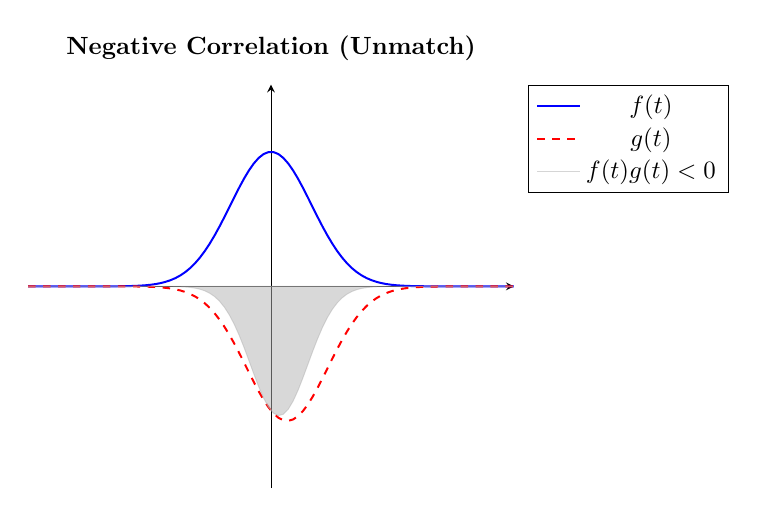
\begin{tikzpicture}[scale=0.9]
\begin{axis}[
    title={\textbf{Negative Correlation (Unmatch)}},
    axis lines=middle, xtick=\empty, ytick=\empty,
    xmin=-3, xmax=3, ymin=-1.5, ymax=1.5,
    legend pos=outer north east]
    
    \addplot[blue, thick, domain=-3:3, samples=100] {exp(-2*x^2)}; \addlegendentry{$f(t)$};
    \addplot[red, dashed, thick, domain=-3:3, samples=100] {-exp(-2*(x-0.2)^2)}; \addlegendentry{$g(t)$};
    
    % Plot the product and fill to axis
    \addplot[black!30, fill=black!30, opacity=0.5, domain=-3:3, samples=100] {exp(-2*x^2) * -exp(-2*(x-0.2)^2)} \closedcycle;
    \addlegendentry{$f(t)g(t) < 0$};
\end{axis}
\end{tikzpicture}
\caption{When $f(t)$ and $g(t)$ are "out of sync," their product $f(t)g(t)$ is always negative, leading to a large negative integral.}
\end{figure}

\subsection{From Inner Product to Convolution}
What, then, is a convolution or a transform?
$$ \text{CWT: } W_f(u, s) = \int_{-\infty}^{\infty} f(t) \psi^* \left( \frac{t-u}{s} \right) dt $$
$$ \text{Fourier: } \hat{f}(\omega) = \int_{-\infty}^{\infty} f(t) e^{-i\omega t} dt $$
Look closely. These are not just inner products. They are \textbf{families of inner products}.

A "transform" like the CWT is not a single calculation; it is an engine for performing a \textbf{sliding inner product}. We aren't just asking, "How similar is our signal $f(t)$ to the wavelet $\psi(t)$?" We are asking a much more powerful question:

"How similar is our signal $f(t)$ to the wavelet $\psi(t)$...
\begin{itemize}
    \item ...when the wavelet is at position $u_1$ and scale $s_1$?" (Calculate inner product)
    \item ...when the wavelet is at position $u_2$ and scale $s_1$?" (Calculate inner product)
    \item ...when the wavelet is at position $u_3$ and scale $s_2$?" (Calculate inner product)
    \item ...for all possible $u$ and $s$?"
\end{itemize}

The resulting "scaleogram" (or "spectrogram" for Fourier) is a giant map where every single pixel's brightness is the result of one inner product, telling you the "similarity score" at that specific time ($u$) and scale ($s$).

This is the bridge. \textbf{An inner product is a similarity score. A transform is a map of similarity scores.}

\newpage

% --- SECTION 1: THE PROBLEM WITH FOURIER ---
\section{The Problem with Fourier: The "Why"}

\subsection{The Fourier Transform: A "What," Not a "When"}
The \textbf{Fourier Transform} is a cornerstone of signal processing. It is built on a profound idea: any complex signal $f(t)$ can be perfectly reconstructed as a sum of simple sine and cosine waves (or complex exponentials).

The transform $\hat{f}(\omega)$ answers the question: "How much of frequency $\omega$ is in my signal?"
$$ \hat{f}(\omega) = \int_{-\infty}^{\infty} f(t) e^{-i\omega t} dt $$
This is, as we just discussed, an inner product. We are asking: "How similar is our signal $f(t)$ to a 'pure' infinite wave $e^{-i\omega t}$?"

\paragraph{The Problem:} The basis functions (sines and cosines) are \textit{infinite in time}. They have perfect "frequency localization" (we know exactly what frequency they are) but zero "time localization" (they exist everywhere, so we don't know \textit{when} they are).

If a signal contains a high-frequency chirp at $t=5$ seconds and a low-frequency rumble at $t=10$ seconds, the Fourier Transform will simply tell you: "This signal contains both high and low frequencies." It cannot tell you \textit{when} they occurred.

\begin{figure}[htbp]
    \centering
    \framebox{\parbox{0.8\textwidth}{\centering
        \vspace{4cm}
        \textbf{Placeholder: Fourier vs. Reality} \\
        \small \textit{Left: A signal with two distinct events in time. \\ Right: Its Fourier transform, showing only two frequency spikes, with all time information lost.}
        \vspace{4cm}
    }}
    \caption{The Fourier Transform identifies \textit{what} frequencies are present, but not \textit{when} or \textit{where} they occur in the signal.}
    \label{fig:fourier_limit}
\end{figure}

\subsection{The Gabor Transform: A First Attempt}
The first logical step to fix this is the \textbf{Short-Time Fourier Transform (STFT)}, or Gabor Transform.
The idea is simple:
\begin{enumerate}
    \item Choose a "window" function $g(t)$ (like a Gaussian) that is localized in time.
    \item Slide this window along your signal $f(t)$.
    \item Perform a Fourier Transform only on the "windowed" part of the signal.
\end{enumerate}
$$ \text{STFT}_f(u, \omega) = \int_{-\infty}^{\infty} f(t) g(t-u) e^{-i\omega t} dt $$
This works! It gives us a \textbf{spectrogram}, which plots frequency content over time.

\paragraph{The New Problem:} This introduces the \textbf{Heisenberg-Gabor Uncertainty Principle}. The size of our window $g(t)$ is fixed.
\begin{itemize}
    \item A \textbf{narrow window} gives good time localization (we know \textit{when} it happened) but poor frequency localization (the smearing from the window blurs all the nearby frequencies).
    \item A \textbf{wide window} gives good frequency localization (we can resolve close frequencies) but poor time localization (we only know it happened "sometime in this wide window").
\end{itemize}
This fixed window size is the critical flaw. We can't analyze high-frequency (short-lived) and low-frequency (long-lived) events with the same "ruler."

% --- SECTION 2: THE WAVELET SOLUTION ---
\section{The Wavelet Solution: A "What" \textit{and} a "When"}
Wavelet analysis solves the fixed-window problem by using a "window" (the wavelet) that can \textit{stretch} and \textit{shrink}.

\subsection{The Mother Wavelet and her "Children"}
We start with a single "Mother Wavelet" function, $\psi(t)$. This function must be localized in both time and frequency and must have a zero mean (it must be a "wave").

$$ \int_{-\infty}^{\infty} \psi(t) dt = 0 $$
A classic example is the Morlet wavelet, which is just a sine wave inside a Gaussian window.

From this one "mother," we generate all our basis functions (the "children") by two operations:
\begin{enumerate}
    \item \textbf{Translation ($u$):} Sliding the wavelet in time, just like in STFT.
    \item \textbf{Scaling ($s$):} Stretching or shrinking the wavelet.
\end{enumerate}
This gives us the wavelet family $\psi_{u,s}(t)$:
$$ \psi_{u,s}(t) = \frac{1}{\sqrt{s}} \psi \left( \frac{t-u}{s} \right) $$
\begin{itemize}
    \item $u$: The position (time).
    \item $s$: The scale (inverse of frequency).
    \item $\frac{1}{\sqrt{s}}$: An energy normalization factor, ensuring all wavelets have the same "strength."
\end{itemize}

\paragraph{This is the key insight:}
\begin{itemize}
    \item \textbf{Small $s$ (High Frequency):} The wavelet is \textit{compressed} (shrunk). This gives a very narrow, high-frequency "ruler"---perfect for pinpointing the \textit{exact time} of a high-frequency spike.
    \item \textbf{Large $s$ (Low Frequency):} The wavelet is \textit{stretched}. This gives a very wide, low-frequency "ruler"---perfect for analyzing the \textit{frequency} of a long, slow oscillation.
\end{itemize}
This is called \textbf{Multi-Resolution Analysis}. Unlike the STFT's fixed window, our analysis "ruler" automatically adapts its time and frequency precision to the feature it's looking for.

\begin{figure}[htbp]
    \centering
    \framebox{\parbox{0.8\textwidth}{\centering
        \vspace{4cm}
        \textbf{Placeholder: Tiling of Time-Frequency Plane} \\
        \small \textit{Left: STFT's uniform grid. Right: Wavelet's adaptive grid, with tall, narrow boxes for high-freq and short, wide boxes for low-freq.}
        \vspace{4cm}
    }}
    \caption{How STFT (left) and Wavelets (right) "see" the time-frequency plane. Wavelets provide high time resolution for high frequencies and high frequency resolution for low frequencies.}
    \label{fig:tiling}
\end{figure}

\subsection{The Continuous Wavelet Transform (CWT)}
The CWT is the full, mathematically-rich version of the wavelet transform. It is defined as the inner product of our signal $f(t)$ with the wavelet family $\psi_{u,s}(t)$ for \textit{all possible} scales $s$ and translations $u$.

$$ W_f(u, s) = \langle f, \psi_{u,s} \rangle = \int_{-\infty}^{\infty} f(t) \frac{1}{\sqrt{s}} \psi^* \left( \frac{t-u}{s} \right) dt $$
The result, $W_f(u,s)$, is a 2D map of "similarity scores." This map is called a \textbf{scaleogram}. It shows the "energy" (the squared coefficient) of the signal at every time $u$ and scale $s$.

\begin{figure}[htbp]
    \centering
    \framebox{\parbox{0.8\textwidth}{\centering
        \vspace{4cm}
        \textbf{Placeholder: Scaleogram of a Chirp Signal} \\
        \small \textit{A 2D plot with Time on the x-axis and Scale/Frequency on the y-axis. A bright, curved line shows the frequency increasing over time.}
        \vspace{4cm}
    }}
    \caption{A scaleogram of a "chirp" signal (where frequency increases). Unlike Fourier, the CWT clearly shows the frequency changing as a function of time.}
    \label{fig:scaleogram}
\end{figure}

\subsection{CWT Code Example: The Chirp Signal}
A "chirp" signal is the perfect test for wavelets, as its frequency content is explicitly time-dependent. We will use the `PyWavelets` library in Python.

\begin{lstlisting}[caption={Python code for CWT of a chirp signal}, label={lst:cwt}]
import numpy as np
import matplotlib.pyplot as plt
import pywt

# 1. Create the signal
fs = 1000 # Sample rate
t = np.linspace(0, 2, 2 * fs)
# A signal that starts at 5 Hz and sweeps up to 50 Hz
chirp_signal = np.sin(2 * np.pi * (5 * t + 11.25 * t**2))
# Add a high-frequency event at t=1.2s
t_event = np.abs(t - 1.2) < 0.05
chirp_signal[t_event] = chirp_signal[t_event] + np.sin(2 * np.pi * 100 * t[t_event])

# 2. Perform the CWT
# We choose 100 scales, from low to high freq
scales = np.arange(1, 100) 
# Use the 'Morlet' wavelet
coef, freqs = pywt.cwt(chirp_signal, scales, 'morl', 1/fs)

# 3. Plot the results
plt.figure(figsize=(12, 8))

# Plot 1: The signal
plt.subplot(2, 1, 1)
plt.plot(t, chirp_signal)
plt.title("Original Signal (Chirp with high-freq event)")
plt.xlabel("Time (s)")
plt.ylabel("Amplitude")

# Plot 2: The Scaleogram
plt.subplot(2, 1, 2)
# We plot the log of the frequencies for better visualization
plt.pcolormesh(t, np.log2(freqs), np.abs(coef)**2, cmap='viridis')
plt.title("CWT Scaleogram (Viridis cmap)")
plt.xlabel("Time (s)")
plt.ylabel("Log(Frequency)")
plt.tight_layout()
plt.show()
\end{lstlisting}

\paragraph{Interpreting the Output:}
The resulting plot (see Figure \ref{fig:scaleogram}) would clearly show:
\begin{enumerate}
    \item A bright, curved line starting at a low frequency and rising over time (the chirp).
    \item A distinct, isolated "blob" of high-frequency energy at $t=1.2$s (the event).
\end{enumerate}
This is a perfect example of time-frequency localization, something the Fourier Transform (Figure \ref{fig:chirp_fourier}) could never do.

\begin{figure}[htbp]
    \centering
    \framebox{\parbox{0.6\textwidth}{\centering
        \vspace{3cm}
        \textbf{Placeholder: Fourier of Chirp} \\
        \small \textit{A 1D plot showing a "smear" of frequencies from 5-50Hz and a spike at 100Hz. No time information.}
        \vspace{3cm}
    }}
    \caption{The Fourier transform of the signal from Listing \ref{lst:cwt}. All time information is lost.}
    \label{fig:chirp_fourier}
\end{figure}

% --- SECTION 3: THE DISCRETE WAVELET TRANSFORM (DWT) ---
\section{The Discrete Wavelet Transform (DWT)}
The CWT is beautiful, but it is also highly redundant and computationally slow. For every time step, we calculate an inner product with hundreds of scales.

The \textbf{Discrete Wavelet Transform (DWT)} provides a fast, efficient, and non-redundant way to compute wavelet coefficients. It is the workhorse behind JPEG2000 image compression, denoising, and data analysis.

\subsection{The Filter Bank Intuition}
The DWT is best understood as a \textbf{filter bank}. At each "level" of decomposition, the DWT splits the signal into two components:
\begin{enumerate}
    \item \textbf{A "Low-Pass" Filter ($g$):} This filter smooths the signal, capturing the slow, low-frequency "Approximation" components.
    \item \textbf{A "High-Pass" Filter ($h$):} This filter sharpens the signal, capturing the fast, high-frequency "Detail" components.
\end{enumerate}
These two filters are mathematically related and are called a \textbf{Quadrature Mirror Filter (QMF)} pair.

\subsection{Multi-Level Decomposition}
Here is the process for a Level-2 DWT:
\begin{enumerate}
    \item \textbf{Level 1:}
    \begin{itemize}
        \item Pass the \textbf{Original Signal} through the low-pass filter $g$ and high-pass filter $h$.
        \item We now have two signals. We "downsample" them (throw away every other sample), because we have twice as much data as we started with.
        \item This yields: \textbf{Level 1 Approximation (cA1)} and \textbf{Level 1 Detail (cD1)}.
    \end{itemize}
    \item \textbf{Level 2:}
    \begin{itemize}
        \item Take the \textbf{cA1} (the "Approximation" from Level 1) and repeat the process.
        \item Pass \textbf{cA1} through the low-pass $g$ and high-pass $h$ filters, then downsample.
        \item This yields: \textbf{Level 2 Approximation (cA2)} and \textbf{Level 2 Detail (cD2)}.
    \end{itemize}
\end{enumerate}
The final DWT representation of the signal is the set of coefficients: $\{ \text{cA2, cD2, cD1} \}$. We have "decomposed" the signal into different frequency bands at different time resolutions.

\begin{figure}[htbp]
    \centering
    \framebox{\parbox{0.9\textwidth}{\centering
        \vspace{5cm}
        \textbf{Placeholder: DWT Filter Bank Diagram} \\
        \small \textit{Flow chart: Signal -> (h, g) -> (Downsample, Downsample) -> (cD1, cA1). Then cA1 -> (h, g) -> (Downsample, Downsample) -> (cD2, cA2).}
        \vspace{5cm}
    }}
    \caption{A 2-level DWT decomposition. The process is iterated on the "Approximation" (cA) coefficients.}
    \label{fig:dwt_diagram}
\end{figure}

\subsection{DWT Code Example: Denoising}
The most famous application of the DWT is denoising. The logic is:
\begin{enumerate}
    \item Perform a DWT of a noisy signal.
    \item \textit{Intuition:} Real signal energy will be concentrated in a few large coefficients, while noise will be spread across many small coefficients.
    \item We apply a "threshold"---setting all coefficients below a certain value to zero.
    \item We perform an \textbf{Inverse DWT (IDWT)} to reconstruct the signal from the "cleaned" coefficients.
\end{enumerate}

\begin{lstlisting}[caption={Python code for DWT denoising}, label={lst:dwt}]
import numpy as np
import matplotlib.pyplot as plt
import pywt

# 1. Create a noisy signal
t = np.linspace(0, 1, 1000)
clean_signal = np.sin(2 * np.pi * 5 * t) + np.sin(2 * np.pi * 12 * t)
noise = 0.5 * np.random.randn(len(t))
noisy_signal = clean_signal + noise

# 2. Decompose the signal
wavelet = 'db4' # Daubechies 4 wavelet
level = 4
coeffs = pywt.wavedec(noisy_signal, wavelet, level=level)

# 3. Threshold the Detail coefficients
# We don't threshold the first coeff (cA4), only cD4, cD3, cD2, cD1
threshold = 0.4
for i in range(1, len(coeffs)):
    coeffs[i] = pywt.threshold(coeffs[i], threshold, mode='soft')

# 4. Reconstruct the signal
denoised_signal = pywt.waverec(coeffs, wavelet)

# 5. Plot the results
plt.figure(figsize=(10, 8))
plt.plot(t, noisy_signal, color='gray', alpha=0.5, label='Noisy')
plt.plot(t, clean_signal, color='black', linestyle='--', label='Original')
plt.plot(t, denoised_signal, color='red', label='Denoised')
plt.legend()
plt.title("DWT Denoising")
plt.show()
\end{lstlisting}

\begin{figure}[htbp]
    \centering
    \framebox{\parbox{0.8\textwidth}{\centering
        \vspace{4cm}
        \textbf{Placeholder: Denoising Plot} \\
        \small \textit{A plot showing the noisy signal, the original clean signal, and the red denoised signal, which closely follows the original.}
        \vspace{4cm}
    }}
    \caption{The output of Listing \ref{lst:dwt}, showing the power of DWT thresholding to recover a clean signal from noise.}
    \label{fig:denoising}
\end{figure}

\section{Conclusion: Which to Use?}
\begin{itemize}
    \item \textbf{Continuous Wavelet Transform (CWT):} Use for analysis, feature extraction, and high-resolution visualization. It is computationally expensive but provides a rich, interpretable map (the scaleogram).
    \item \textbf{Discrete Wavelet Transform (DWT):} Use for applications requiring speed and efficiency, such as compression (JPEG2000), denoising, and real-time data processing. It is a fast, non-redundant, and perfectly invertible transform.
\end{itemize}

Wavelet analysis is a fundamental tool that bridges the gap between pure time-domain and pure frequency-domain analysis, allowing us to finally see \textit{what} is happening \textit{when}.

\end{document}
